\chapter{METODOLOGI}
\label{chap:metodologi}

\section{Kerangka \textit{CRISP-DM}}
\label{sec:crispdm}
Proyek ini mengikuti \textit{Cross-Industry Standard Process for Data Mining} (CRISP-DM) \cite{chapman2000}, yaitu enam tahap yang dapat berulang (Gambar~\ref{fig:crispdm}). Tabel~\ref{tab:crispdm} memetakan setiap tahap ke penerapannya pada proyek ini, dan Gambar~\ref{fig:alur-kerja} menunjukkan alur data antar-\textit{notebook}.

\begin{figure}[!htb]
\centering
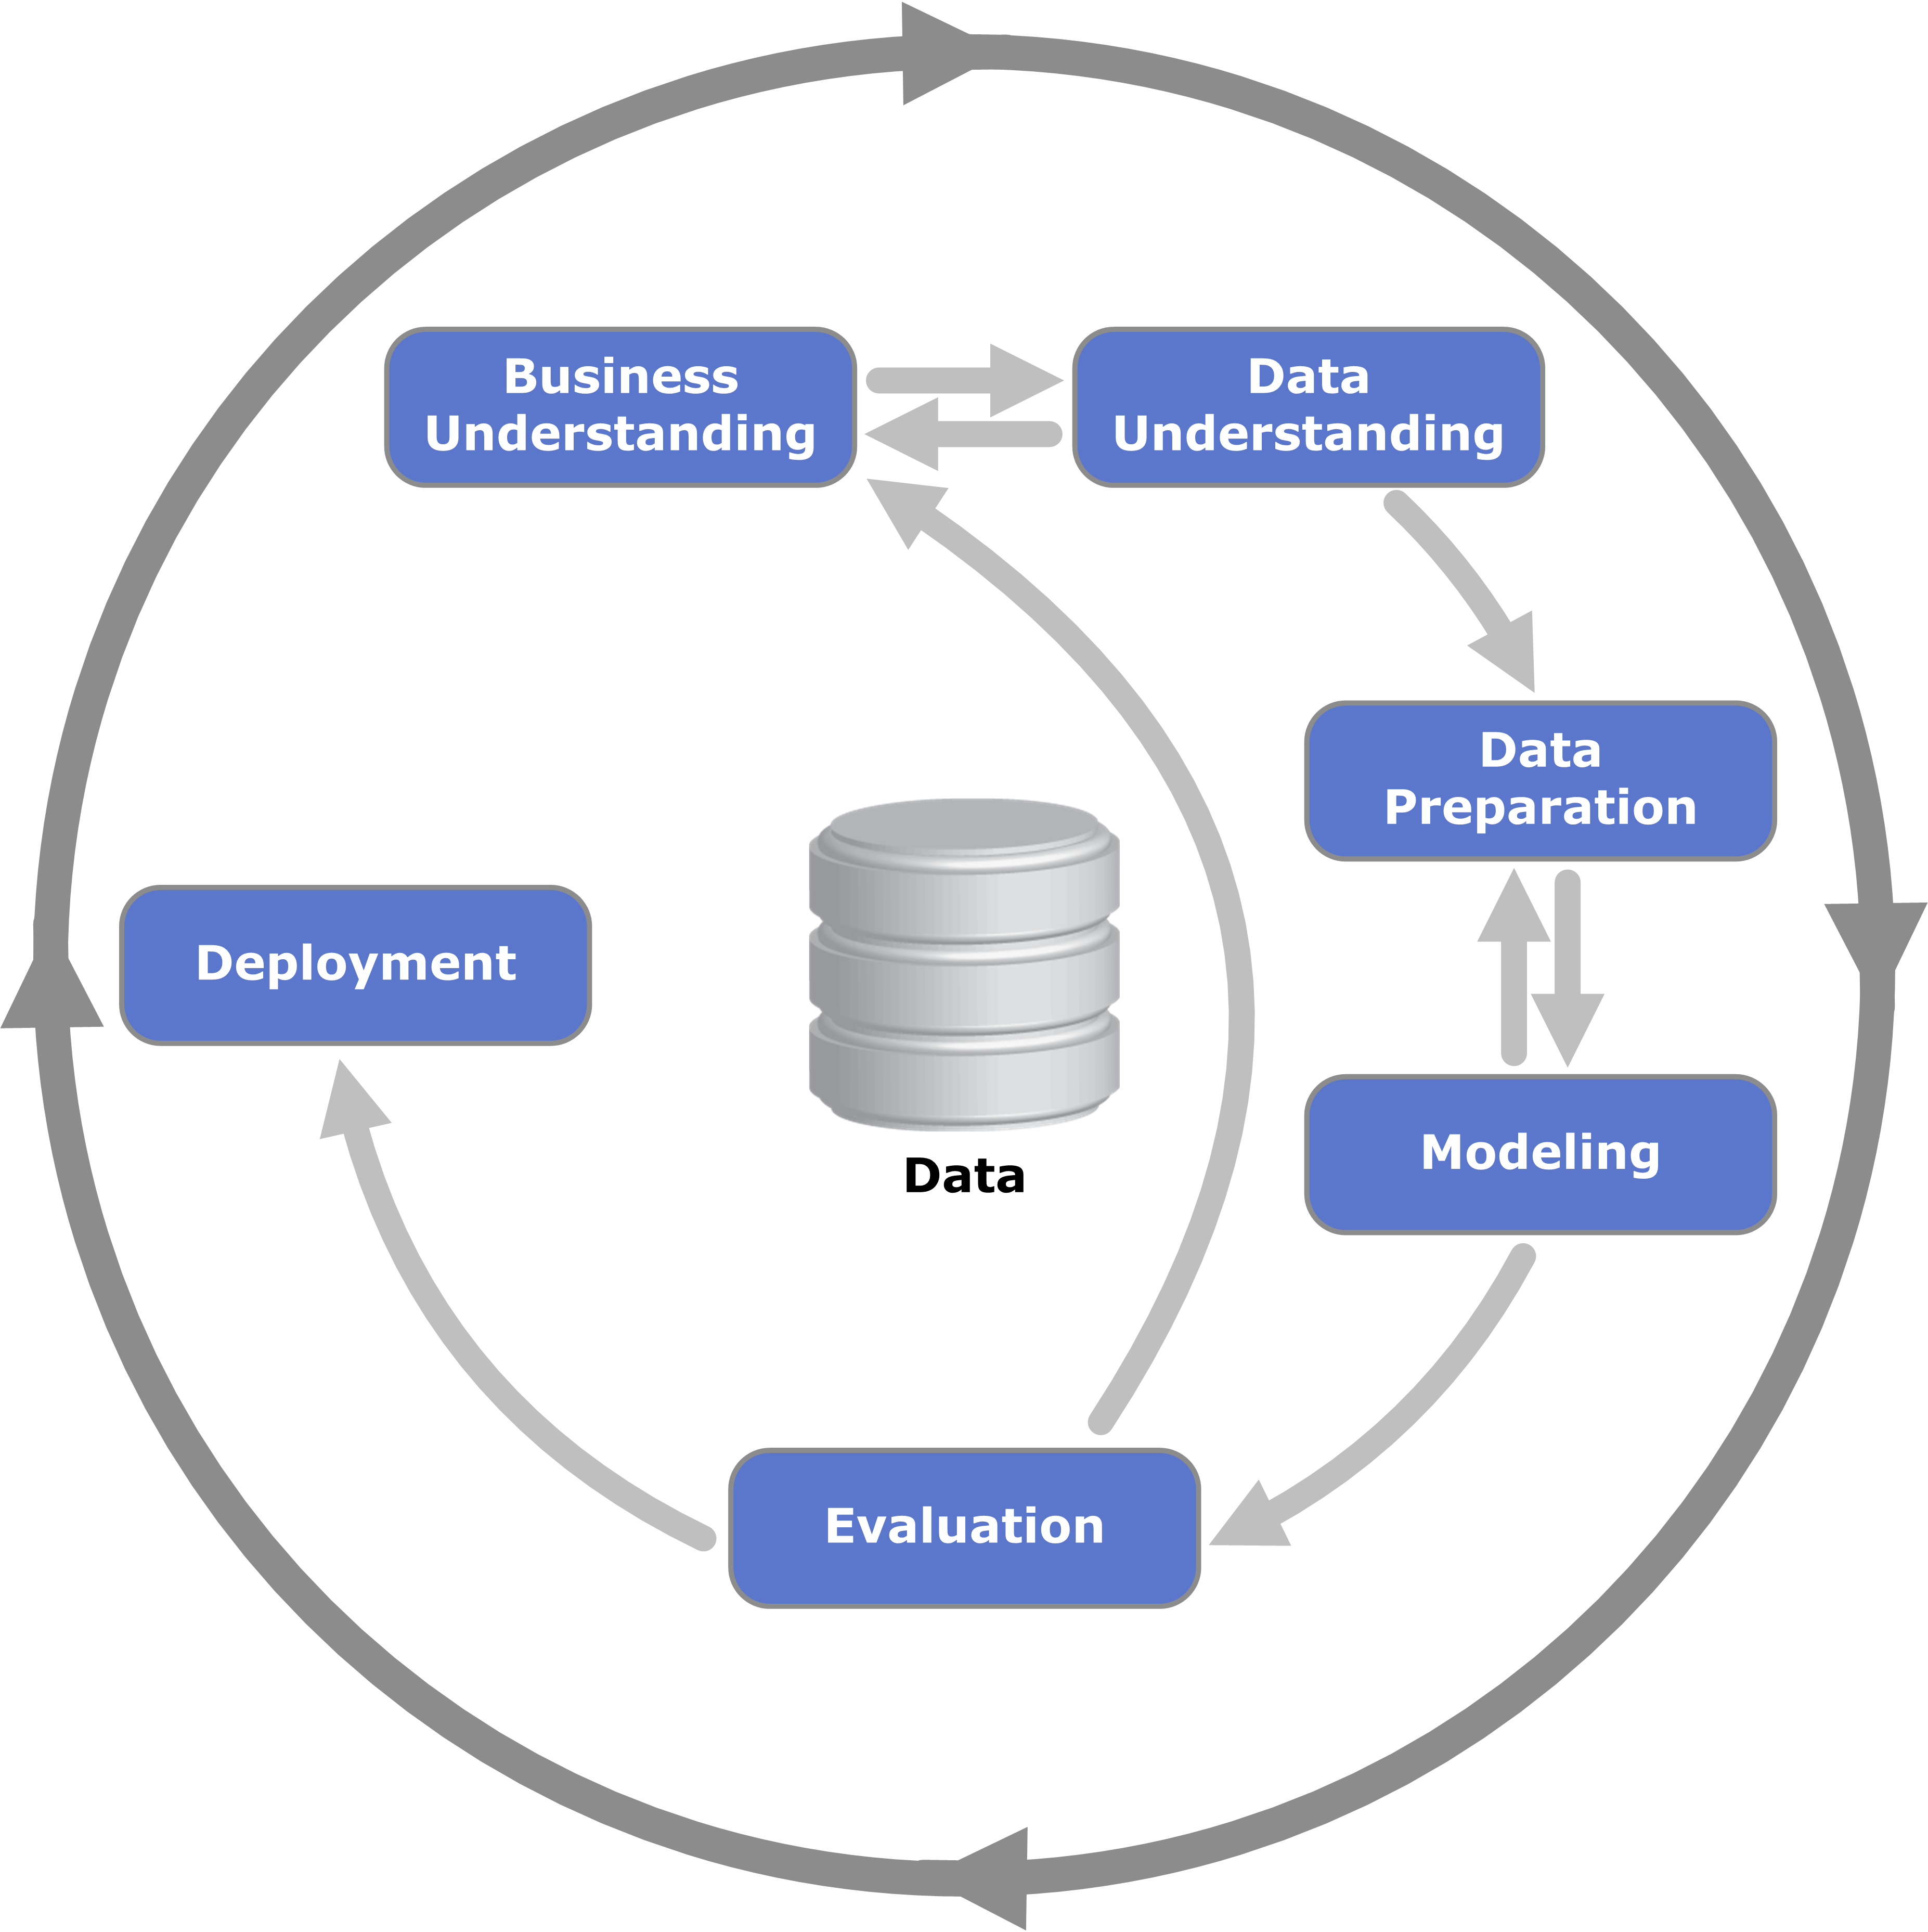
\includegraphics[width=0.45\textwidth]{images/crispdm.png}
\caption{Proses CRISP-DM (Jensen 2012)}
\label{fig:crispdm}
\end{figure}

\begin{table}[!htb]
\caption{Penerapan CRISP-DM pada proyek}
\label{tab:crispdm}
\small
\begin{tabularx}{\textwidth}{@{}p{3.6cm}Xp{1.9cm}@{}}
\toprule
\textbf{Tahap} & \textbf{Penerapan pada proyek} & \textbf{Bab} \\
\midrule
\textit{Business Understanding} & Menentukan tujuan, ukuran popularitas, dan pertanyaan penelitian & I \\
\midrule
\textit{Data Understanding} & Mengeksplorasi struktur dan \textit{key} DBLP, statistik data, dan popularitas konferensi & II, IV, V \\
\midrule
\textit{Data Preparation} & \textit{Preprocessing} lima tahap dan pembentukan dua \textit{transactional database} & IV, VI \\
\midrule
\textit{Modeling} & Apriori, FP-Growth, dan \textit{association rules} & VII, VIII \\
\midrule
\textit{Evaluation} & Validasi hasil, perbandingan performa, dan analisis temporal & IX, X \\
\midrule
\textit{Deployment} & Laporan dan presentasi & XI, XII \\
\bottomrule
\end{tabularx}
\end{table}

\begin{figure}[!htb]
\centering
\figtikz[7cm]{fig-alur-kerja}
\caption{Alur data dan \textit{notebook}}
\label{fig:alur-kerja}
\end{figure}

\section{\textit{Business Understanding}}
Tujuan proyek adalah mengetahui konferensi yang paling aktif dan konferensi yang sering dipilih oleh peneliti yang sama. Popularitas konferensi diukur dari aktivitas publikasi, yaitu jumlah publikasi dan jumlah penulis unik, sedangkan keterkaitan antarkonferensi diukur dari kemunculan bersama pada riwayat publikasi penulis.

\section{\textit{Data Understanding}}
\label{sec:ekstraksi}
Tahap ini terdiri atas tiga kegiatan.
\begin{enumerate}
\item Ekstraksi: \textit{dump} dibaca secara \textit{streaming} dan hanya \textit{record} \texttt{inproceedings} 2015--2025 yang disimpan (2.004.202 \textit{record}).
\item Seleksi: \textit{record} harus bertag \texttt{inproceedings}, ber\textit{key} \texttt{conf/}, dan terbit pada 2015--2025. Syarat \texttt{conf/} ditambahkan karena 3.161 \textit{record} bertag \texttt{inproceedings} berasal dari prosiding acara kecil pada seri jurnal (\texttt{journals/corr}, \texttt{journals/entcs}, dan \texttt{books/sp}) yang menyatu menjadi \textit{venue} palsu dan tidak mungkin mencapai \textit{min\_sup}.
\item Analisis popularitas: pertumbuhan dinyatakan dengan \textit{compound annual growth rate} (CAGR) 2015--2024, dan tahun 2025 tidak dipakai karena datanya belum lengkap. Keselarasan dua peringkat diukur dengan korelasi Spearman, dan dampak penggabungan \textit{workshop} ke konferensi induk diuji dengan menghitung ulang peringkat tanpa \textit{workshop}.
\end{enumerate}

\section{\textit{Data Preparation}}
\label{sec:preprocessing}
\subsection{\textit{Preprocessing}}
Tabel~\ref{tab:prepro} merangkum lima tahap \textit{preprocessing}, yang masing-masing dikerjakan pada salinan data mentah.

\begin{table}[!htb]
\caption{Tahapan \textit{preprocessing}}
\label{tab:prepro}
\small
\begin{tabularx}{\textwidth}{@{}p{3.3cm}XX@{}}
\toprule
\textbf{Tahap} & \textbf{Perlakuan} & \textbf{Alasan} \\
\midrule
Konsistensi tahun & Konversi teks ke bilangan bulat dan validasi rentang 2015--2025 & \texttt{year} bertipe teks pada XML \\
\midrule
\textit{Missing values} & Membuang makalah tanpa penulis & Tidak dapat masuk transaksi dan umumnya bukan makalah \\
\midrule
Seleksi dan normalisasi \textit{venue} & Hanya \textit{key} \texttt{conf/}; \textit{venue} = segmen kedua \textit{key} & Sesuai Subbab~\ref{sec:key}; \textit{booktitle} tidak konsisten \\
\midrule
Duplikat & Membuang \textit{key} ganda, lalu judul, tahun, dan \textit{venue} ganda & Satu makalah tidak boleh terhitung dua kali \\
\midrule
Normalisasi penulis & Normalisasi Unicode NFKC dan spasi; sufiks DBLP dipertahankan; dipecah per penulis & Menyeragamkan nama tanpa menggabungkan orang berbeda \\
\bottomrule
\end{tabularx}
\end{table}

Hasil \textit{preprocessing} disimpan dalam format Parquet, yang lebih kecil dan lebih cepat dibaca daripada CSV serta mempertahankan tipe data. Tiga tabel dihasilkan: \texttt{raw} (2.004.202 makalah), \texttt{clean} (1.997.244 makalah) untuk perhitungan per makalah, dan \texttt{paper\_author} (7.870.902 pasangan makalah-penulis) untuk perhitungan per penulis dan pembentukan transaksi.

\subsection{\textit{Transactional Database}}
Dua \textit{database} dibentuk dari \texttt{paper\_author} dengan \textit{venue} sebagai item (Tabel~\ref{tab:def-db}). Setiap transaksi berupa himpunan \textit{venue} unik, sehingga dua makalah pada \textit{venue} yang sama dalam satu transaksi hanya menghasilkan satu item. Bentuk ini sesuai dengan tujuan analisis, yaitu daftar konferensi tempat penulis menerbitkan makalah, dan jumlah makalah per transaksi tetap tersimpan pada kolom \texttt{n\_paper}.

\begin{table}[!htb]
\caption{Definisi dua \textit{transactional database}}
\label{tab:def-db}
\small
\begin{tabularx}{\textwidth}{@{}p{2.8cm}XX@{}}
\toprule
 & \textbf{\textit{Author-based}} & \textbf{\textit{Author-year-based}} \\
\midrule
Satu transaksi & Satu penulis & Satu kombinasi penulis dan tahun \\
\midrule
Item & \textit{Venue} yang diterbitkan penulis selama 2015--2025 & \textit{Venue} yang diterbitkan penulis pada tahun itu \\
\midrule
Dipakai pada & \textit{Frequent pattern mining} dan \textit{association rules} & Analisis temporal \\
\bottomrule
\end{tabularx}
\end{table}

\subsection{Struktur Data}
\label{sec:struktur-data}
Kedua \textit{database} dibentuk dari satu tabel panjang \texttt{(tid, item)} yang disimpan di disk agar isinya konsisten, lalu diturunkan menjadi dua bentuk di memori (Gambar~\ref{fig:satu-sumber}). Kesetaraan kedua bentuk diperiksa pada jumlah transaksi, jumlah pasangan, ukuran tiap transaksi, dan isi 2.000 transaksi acak. Tabel~\ref{tab:bentuk} membandingkan bentuk yang dipertimbangkan.

\begin{figure}[!htb]
\centering
\figtikz[6.6cm]{fig-satu-sumber}
\caption{Struktur data \textit{transactional database}}
\label{fig:satu-sumber}
\end{figure}

\begin{table}[!htb]
\caption{Bentuk representasi \textit{database} \textit{author-based}}
\label{tab:bentuk}
\small
\begin{tabularx}{\textwidth}{@{}p{2.8cm}XlX@{}}
\toprule
\textbf{Bentuk} & \textbf{Struktur} & \textbf{Memori} & \textbf{Kegunaan} \\
\midrule
Horizontal & \textit{List} \textit{frozenset} berkode integer & 270 MB & Masukan Apriori dan FP-Growth \\
\midrule
\textit{Sparse} CSR & Matriks 0 dan 1 transaksi $\times$ item & 35 MB & Statistik dan validasi \texttt{mlxtend} \\
\midrule
\textit{Dense} & Matriks 0 dan 1 penuh & 8,0 GB & Tidak dibuat \\
\bottomrule
\end{tabularx}
\end{table}

\subsection{Aturan \textit{Mining}}
\label{sec:aturan-mining}
Empat aturan ditetapkan agar hasil konsisten.
\begin{enumerate}
\item Item yang tidak \textit{frequent} dipangkas sebelum \textit{mining}.
\item Penyebut \textit{support} adalah seluruh transaksi, sedangkan transaksi berisi kurang dari dua item \textit{frequent} cukup dilewati untuk \textit{itemset} berukuran dua ke atas.
\item Waktu eksekusi tidak mencakup pemuatan Parquet dan pembentukan \textit{database} horizontal, tetapi mencakup pembentukan FP-\textit{tree} pada FP-Growth.
\item Hasil setiap algoritma divalidasi dengan \texttt{mlxtend} \cite{raschka2018}: \textit{itemset} dan \textit{support} harus identik.
\end{enumerate}

\section{\textit{Modeling}}
Apriori dan FP-Growth dijalankan pada \textit{author-based database}, lalu \textit{association rules} dibangkitkan dari \textit{frequent itemsets} yang dihasilkan. Konfigurasi eksperimen dirangkum pada Tabel~\ref{tab:konfigurasi}.

\begin{table}[!htb]
\caption{Konfigurasi eksperimen}
\label{tab:konfigurasi}
\small
\begin{tabularx}{\textwidth}{@{}p{4.6cm}X@{}}
\toprule
\textbf{Parameter} & \textbf{Nilai} \\
\midrule
\textit{Database} \textit{mining} dan perbandingan performa & \textit{Author-based} (1.821.757 transaksi) \\
\midrule
\textit{min\_sup} & 0,1\%, 0,5\%, 1\%, dan 2\% \\
\midrule
\textit{min\_conf} & 50\% \\
\midrule
Ukuran \textit{rule} & \textit{Support}, \textit{confidence}, dan \textit{lift} \\
\midrule
Pengulangan waktu & Tiga kali per kombinasi, dilaporkan median dan rentangnya \\
\midrule
\textit{Database} analisis temporal & \textit{Author-year-based}, empat periode: 2015--2017, 2018--2020, 2021--2023, dan 2024--2025 \\
\midrule
\textit{min\_sup} analisis temporal & 0,01\%, 0,02\% (utama), dan 0,05\% \\
\bottomrule
\end{tabularx}
\end{table}

\section{\textit{Evaluation}}
Evaluasi mencakup tiga hal. Pertama, validasi hasil kedua algoritma terhadap \texttt{mlxtend}. Kedua, perbandingan Apriori dan FP-Growth berdasarkan jumlah \textit{frequent itemsets}, jumlah \textit{rules}, dan waktu eksekusi pada setiap \textit{min\_sup}. Ketiga, perbandingan \textit{rules} antarperiode pada analisis temporal, yaitu yang bertahan, hilang, dan muncul.

\section{\textit{Deployment}}
Hasil disajikan dalam laporan ini dan presentasi. Seluruh kode dan \textit{notebook} dapat dijalankan ulang berurutan dari \textit{dump} DBLP.
